\documentclass[t]{beamer}

\mode<handout>
{
  \usepackage{pgf}
  \usepackage{pgfpages}

\pgfpagesdeclarelayout{4 on 1 boxed}
{
  \edef\pgfpageoptionheight{\the\paperheight} 
  \edef\pgfpageoptionwidth{\the\paperwidth}
  \edef\pgfpageoptionborder{0pt}
}
{
  \pgfpagesphysicalpageoptions
  {%
    logical pages=4,%
    physical height=\pgfpageoptionheight,%
    physical width=\pgfpageoptionwidth%
  }
  \pgfpageslogicalpageoptions{1}
  {%
    border code=\pgfsetlinewidth{2pt}\pgfstroke,%
    border shrink=\pgfpageoptionborder,%
    resized width=.5\pgfphysicalwidth,%
    resized height=.5\pgfphysicalheight,%
    center=\pgfpoint{.25\pgfphysicalwidth}{.75\pgfphysicalheight}%
  }%
  \pgfpageslogicalpageoptions{2}
  {%
    border code=\pgfsetlinewidth{2pt}\pgfstroke,%
    border shrink=\pgfpageoptionborder,%
    resized width=.5\pgfphysicalwidth,%
    resized height=.5\pgfphysicalheight,%
    center=\pgfpoint{.75\pgfphysicalwidth}{.75\pgfphysicalheight}%
  }%
  \pgfpageslogicalpageoptions{3}
  {%
    border code=\pgfsetlinewidth{2pt}\pgfstroke,%
    border shrink=\pgfpageoptionborder,%
    resized width=.5\pgfphysicalwidth,%
    resized height=.5\pgfphysicalheight,%
    center=\pgfpoint{.25\pgfphysicalwidth}{.25\pgfphysicalheight}%
  }%
  \pgfpageslogicalpageoptions{4}
  {%
    border code=\pgfsetlinewidth{2pt}\pgfstroke,%
    border shrink=\pgfpageoptionborder,%
    resized width=.5\pgfphysicalwidth,%
    resized height=.5\pgfphysicalheight,%
    center=\pgfpoint{.75\pgfphysicalwidth}{.25\pgfphysicalheight}%
  }%
}


  \pgfpagesuselayout{4 on 1 boxed}[a4paper, border shrink=5mm, landscape]
  \nofiles
}

%% Language and font encodings
\usepackage[english]{babel}
\usepackage[utf8x]{inputenc}
\usepackage[T1]{fontenc}

\usetheme{Madrid}
\usecolortheme{beaver}

%% Useful packages
\usepackage{amsmath}
\usepackage{graphicx}

\usepackage{enumitem}

% full page itemieze
\newenvironment{fpi}
  {\itemize[nolistsep,itemsep=\fill]}
  {\vfill\enditemize}

\newcommand{\img}[1]{
\vfill
\includegraphics[width=\textwidth,height=0.5\textheight,keepaspectratio]{#1}
\vfill
} 


\title{Approximating Slopes of Tangent Lines  \\
 Introduction to Limits}
\date{January 31, 2017 \\ 9:35 - 10:50 AM}

\begin{document}
\frame{\titlepage}


\begin{frame}{Outline}
\begin{fpi}
\item Review of inverse functions and logs
\item Tangent lines
\item Average velocity
\item Instantaneous velocity
\item Estimating slopes of tangent lines
\item Limits
\end{fpi}
\end{frame}

\begin{frame}{Tangent lines}
The tangent line to a graph $y = f(x)$ at a point $x_0$ is the line
that barely touches the graph at $(x_0, f(x_0))$.
\end{frame}

\begin{frame}{Average velocity}
Given  a function $f(t)$ describing the position of an object
at time $t$, its average velocity between times $t_0$ and $t_1$ is
$$ v_{ave} = \frac{ f(t_1) - f(t_0)} {t_1 - t_0} $$
\end{frame}

\begin{frame}{Instantaneous velocity}
Given  a function $f(t)$ describing the position of an object
at time $t$, its instantaneous velocity at time $t_0$ is the 
slope of the tangent line at $t = t_0$.
\end{frame}

\begin{frame}{Estimating slopes of tangent lines}
Two ways to estimate the slope of the tangent line at $x = x_0$:
\begin{itemize}
\item Secant lines approaching $x_0$ from the right
\item Secant lines approaching $x_0$ from the left
\end{itemize}
\end{frame}


\begin{frame}{Estimating slopes}
Estimate the slope of the tangent line at $t = 1$ using each of the 4 other 
data points.
\begin{table}
\begin{tabular}{c c}
t (sec) & dist (m) \\
5 & 22 \\
2 & 1 \\
1.1 & -1.79 \\
1.01 & -1.9799 \\
1 & 2 
\end{tabular}
\end{table}
\end{frame}

\begin{frame}{Estimating slopes}
The distance an airplane which is taking off has
travelled is given by the formula
$$D(t)  = 3t^2 - t + 5 $$
Estimate the velocity of the airplane at $t = 3$ by using
time intervals starting at $t = 3$ and lasting $1$, $. 5$, $. 1$,
and $. 01$ seconds.
\end{frame}


\begin{frame}{Estimating slopes}
An electron moves along a wire in an AC circuit according to
the formula
$$x(t) = 5 \sin \left( \frac{\pi t}{2} \right) $$
Estimate the velocity of the electron when $t = $ by using
the time intervals $[2,4]$, $[3,4]$, $[3.5,4]$, $[3.9,4]$, and
$[3.99,4]$.
\end{frame}

\begin{frame}{Limits}
To take the limit of a function $y = f(x)$ at the point $x = a$, we
look at the $y$-values as the $x$-values get closer to $a$.
\end{frame}

\begin{frame}{Example}
Let 
$$f(x) = x^2 + 2$$

To calculate the limit at $x = 2$, we compute the following values:

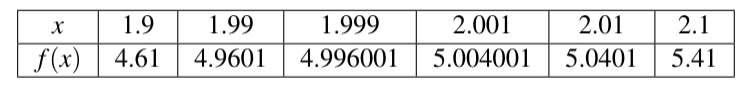
\includegraphics[width=\textwidth,keepaspectratio]{limits}

We say the limit as $x$ approaches $2$ equals 5, or 
$\displaystyle \lim_{x\to 2}f(x) = 5$.
\end{frame}

\begin{frame}{Remark}
Limits are important when the graph displays unusual behavior around 
the point in question.  On the previous example, we could have just
plugged $x = 2$ into the function.
\end{frame}

\begin{frame}{Removable discontinuity example}
Let 
$$f(x) = \frac{x^2 - 9}{x-3}$$

To calculate the limit at $x = 3$, we compute the following values:

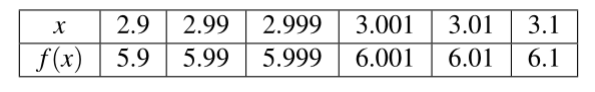
\includegraphics[width=\textwidth,keepaspectratio]{limits2}

So $\displaystyle \lim_{x\to 3}f(x) = 6$.
\end{frame}

\begin{frame}{Limits of piecewise functions}
Let 
$$ f(x) = \begin{cases}
x^2 - 1, & x < 0 \\
2x + 5, & x \ge 0 
\end{cases}
$$
\end{frame}

\begin{frame}{Left and right-handed limits}
\begin{fpi}
\item In this case, we write 
$$ \lim_{x \to 0 ^-} f(x) = $$
\item $$ \lim_{x \to 0 ^+} f(x) = $$
\item The actual (two-sided) limit $\displaystyle \lim_{x \to 0} f(x)$ 
only exists if the left and right-handed limits are equal.  
They are not, so  the limit DNE (does not exist)
\end{fpi}
\end{frame}

\begin{frame}{Example}
\img{pwlimits}
\end{frame}

\begin{frame}{Example}
\img{pwlimits2}
\end{frame}

\end{document}
